% !TEX encoding = UTF-8 Unicode
% ch04：预测端——λ_max 代理阶梯（中文深度解读片段）
\section{预测端：\lmax 的代理阶梯}
\label{sec:ch04}

\begin{keybox}{先抓住本章的五件事}
\begin{itemize}
  \item 论文把廉价尖锐度量组织成一条\textbf{阶梯}：0 次 HVP 的范数 / $\gamma$ 代理 $\to$ 1 次 HVP 的梯度瑞利商 $\lhatg$ $\to$ 中位 4--11 次 HVP 的热启动精确测量（ground truth）。
  \item Tier-0 零计算代理是\textbf{归一化族依赖且种子不稳定}的：plain 网各层范数 Pearson $0.65$--$0.71$（last-hidden 最优，$10/14$ runs）；BN 下相关由正转负（$-0.8$），信号转移到 $\gamma$，但多种子去趋势仅 $+0.247\pm0.340$、CI 跨零；LN/Transformer 上触顶于 $\|\mathbf{g}\|$（$+0.52$）。
  \item 单 HVP 梯度瑞利商 $\lhatg=\mathbf{g}^{\top}H\mathbf{g}/\mathbf{g}^{\top}\mathbf{g}$ 在 ResNet 上全程去趋势 $r=+0.898\pm0.141$，EoS 体制（$|\cos(\mathbf{g},\vtope)|>0.7$）内 $+0.981\pm0.030$，近乎精确。
  \item 约 $17\%$ 的相对差距\textbf{不是噪声}，而是瑞利下界的预期松弛（Rayleigh slack，下界与真值的固有差距）：EoS 体制内对齐 $|\cos|\!\to\!0.85$--$0.9$，故 $\cos^{2}\!\approx\!0.8$。
  \item 监测探针是\textbf{原始梯度而非动量更新}：对齐 $0.563\pm0.017$ 对 $0.511\pm0.024$，EoS 相对误差 $0.169\pm0.026$ 对 $0.238\pm0.026$，两个 CI 均不重叠。
\end{itemize}
\end{keybox}

\noindent 本章对应论文第 4 节（Predictors: a $\lmax$ proxy
ladder），是论文“半张成功”的那一半：摘要里的第一句结论——廉价尖锐度\emph{预测器}能可靠跟踪
$\lmax$——的全部证据都在这里。教程第 9
节已经给出“权重范数可以当尖锐度代理”的入门版；论文在这一节做的是把入门版升级为完整的\textbf{代理阶梯}：给出每一层的成本、每一层的可靠性刻画（在哪种归一化族、哪个训练阶段、哪种采样密度下可信），并在阶梯的甜蜜点（sweet spot，成本--精度权衡的最优档位）上交付一个“部署就绪”的单
HVP
监测器。读完本章你会看到：预测端的成功不是“找到一个好代理”，而是\textbf{刻画出一张何时信任哪个代理的地图}。

\subsection{阶梯总览：三个成本档位}
\label{sec:ch04-ladder}

先把阶梯本身画出来。衡量的成本单位是 HVP（海森--向量积，一次双重反传，教程第 3
节讲过）：

\begin{table}[!ht]
\centering\small
\caption{论文的 \lmax 代理阶梯。成本从零到精确；本章自下而上逐层检验。}
\label{tab:ch04-ladder}
\begin{tabular}{lccl}
\toprule
档位 & 量 & 成本 & 角色 \\
\midrule
Tier-0 & 各层 $\|\mathbf{W}\|$、$\|\gamma\|$、$\|\mathbf{g}\|$ & 0 HVP & 免费的粗监测，可靠性依赖归一化族 \\
Tier-1 & $\lhatg=\mathbf{g}^{\top}H\mathbf{g}/\mathbf{g}^{\top}\mathbf{g}$（或 $\lhatd$） & 1 HVP & 论文交付的部署级监测器 \\
精确顶端 & 热启动幂迭代（Ramasinghe 等 2026） & $\sim$5 HVP（中位 4--11） & ground truth 尺子 \\
（参照） & $\lambda_c$ 线搜（Kalra 等 2026） & 5--6 次前传 & 另一条精确路径，无需 HVP \\
\bottomrule
\end{tabular}
\end{table}

这条阶梯的设计逻辑值得点破：精确顶端是\textbf{借来的尺子}（解读第
\ref{sec:ch02-exact} 节），它的存在让下面每一层都可以被定量评价——不是“看起来像
$\lmax$”，而是“与真值的相关是多少、差多少、为什么差”。Tier-0
是免费的，但要回答“在哪种网络上可信”；Tier-1 花一次
HVP，论文主张它是实践者的甜蜜点。注意 $\lhatg$
的数学身份：在局部二次型（quadratic form，形如 $\mathbf{x}^{\!\top}\!H\mathbf{x}$
的标量；“局部二次型”即把损失面在当前参数附近近似成二次函数——泰勒
展开截到二阶）下它\emph{代数上等于}临界尖锐度 $\lambda_c$（Kalra 等
2026 的结果 2.1，本文不据为新颖，只在二次型上验证到 $\pm0.5\%$，见解读第
\ref{sec:ch02-directional} 节）；它是 $\lmax$ 的\textbf{瑞利下界}，当且仅当
$\mathbf{g}$ 与 $\vtope$ 对齐时取等。这个“下界 +
取等条件”的结构，是理解本章所有数字的钥匙。

\subsection{Tier-0：零计算代理的地图与裂缝}
\label{sec:ch04-tier0}

\textbf{plain 网络上，教程结论被细化。} 在 tanh MLP 上（主 teacher--student run
加 13 个难度 / lr / 宽度扫描，共 14 个 run），\emph{每一层}的权重范数都与
$\lmax$ 相关（平均 Pearson $0.65$--$0.71$），其中\textbf{last-hidden 层最优}（在
$10/14$ 个 run 里是最佳单层）。这细化了 Li 等 (2022)
的“输出层范数代理”：输出层并不是唯一的诊断层，最后一隐藏层反而是更强的跟踪者。教程第
9 节若给你留下“看输出层就行”的印象，这里应修正为“看最后两层都行、last-hidden
略优”。

\textbf{BatchNorm 下，地图整个翻面。}先把 BatchNorm 与它的 $\gamma$
说清楚。BN 层插在卷积 / 线性层之后，对\emph{每个通道}的激活在 batch
维上做标准化（减均值、除以标准差），随后再施加一个\emph{逐通道}的仿射
变换 $y=\gamma\odot\hat{x}+\beta$：$\hat{x}$ 是标准化后的激活，
$\odot$ 是逐元素乘，$\gamma$（缩放）与 $\beta$（平移）是该层仅有的
两个可学习参数（即 PyTorch 里 BN 模块的 \texttt{weight} 与
\texttt{bias}）。全文的“$\|\gamma\|$”指把网络中\emph{所有} BN 层的
$\gamma$ 向量首尾拼接成一个长向量后取 $\ell_2$ 范数——与 plain 网络
里 $\|\mathbf{W}\|$ 完全同构的一个“网络有多大的尺度”指标。

在这个基础上，翻面就有了第一性解释。BN 网络上权重范数与 $\lmax$ 的
相关\textbf{由正转负}至 $-0.8$，机制是 BN 的\textbf{尺度不变性}：把
某层权重 $\mathbf{W}$ 整体放大 $c$ 倍，紧跟其后的 BN 会在标准化时把这
个放大\emph{除回去}——网络函数与 BN 之后的曲率几乎不变。plain 网络里
“$\|\mathbf{W}\|$ 大 $\Rightarrow$ 激活大 $\Rightarrow$ 曲率大”的传导
链被 BN 当中一截剪断：权重范数可以涨落而不触碰曲率，曲率生长也不再
需要权重范数配合——两个量由此\textbf{解耦}，相关自然塌掉甚至翻负。
但“网络的尺度在长个子”这件事本身没有消失，只是换了记账的参数：
$\gamma$ 逐通道直接乘在（标准化后的）激活上，$\gamma$ 变大、下游激活
与损失曲率同步放大。于是在 BN 体制下，承载尺度 / 尖锐度信息的参数从
$\mathbf{W}$ 换成了 $\gamma$——这正是第五章 C2 $\gamma$-帽的设计依据，
也是教程读者在项目 README 里见过的“范数帽优化器在 BN 网络上不工作”
的机制根源：它的传感器在 BN 体制下读的是反号的信息。

\textbf{但接住信号的 $\gamma$ 本身是坏温度计。}
多种子（$n{=}5$）之后，BN-$\gamma$ 代理的去趋势相关只有
$+0.247\pm0.340$，逐种子从 $+0.55$ 摆到
$-0.05$，\textbf{置信区间跨零}。也就是说：单看某一个
seed，你可能得到一个“还不错”的 $+0.55$，并据此相信 $\|\gamma\|$
是可靠代理——多种子 CI 揭示这只是运气。这是论文统计规范（解读第
\ref{sec:ch03-stats} 节）第一次展现出裁决力。

\textbf{LayerNorm / Transformer 上，零计算代理触顶。} LayerNorm 是
Transformer 一侧的对应物：对\emph{每个样本}在特征维上做标准化、再施加
自己的 $\gamma/\beta$ 仿射——不依赖 batch 统计（因此没有 BN 那种跨
样本耦合与训练 / 推断行为差异），但同样把权重尺度与曲率解耦。在
ViT-tiny 与 ConvNeXt-atto 上，最佳零计算代理是\textbf{梯度范数}
$\|\mathbf{g}\|$（两个架构上同为 $+0.52$），但只比 $\|\gamma\|$ /
$\|W_{\mathrm{attn}}\|$（约 $0.44$）高约 $0.08$；把注意力权重与 MLP
权重拆开分别测也无济于事。所有零计算候选挤在 $0.44$--$0.52$
的窄带里——对监测来说，这点区分度实在拿不出手。

\textbf{采样密度本身是一个隐藏变量。} 论文在此插入了一个方法学警示：一个 16
点的去趋势相关，可以仅因窗口选择而摆动
$\pm0.25$——原因是不对称的动态尺度：$\|\gamma\|$ 全程移动不足 $1\%$，而 $\lmax$
摆动 $20\times$。密集采样后该相关稳定在 $+0.44$。这个警示与解读第
\ref{sec:ch03-stats}
节的去趋势理由是一体两面：当被相关的两条曲线漂移速度差两个数量级时，任何带窗口的去趋势都会变得对采样相位敏感。实践含义：\textbf{不要在稀疏采样的
run 上比较代理优劣}。

\subsection{单 HVP 梯度瑞利商 \lhatg：EoS 体制内近乎精确}
\label{sec:ch04-rayleigh}

现在上阶梯的第二层。$\lhatg=\mathbf{g}^{\top}H\mathbf{g}/\mathbf{g}^{\top}\mathbf{g}$
只花\textbf{一次} HVP（算 $H\mathbf{g}$，再做两个内积），它在 ResNet-18
上的成绩（表~\ref{tab:ch04-proxy}）是本章的核心数字：全程去趋势
$r=+0.898\pm0.141$；限定在 \textbf{EoS 体制}（判据
$|\cos(\mathbf{g},\vtope)|>0.7$）内，$r=+0.981\pm0.030$。

这组数字里最有教学价值的是\textbf{误差的结构}。$\lhatg$ 相对 $\lmax$
系统性地低约 $17\%$——论文没有把这 $17\%$
当作说不清的残差轻松放过，而是指出它正是\textbf{瑞利下界的预期 slack}（Rayleigh
slack，下界读数与真值的固有差距）。来历一句话讲清：把 $\mathbf{g}$
分解到海森的各特征方向上，瑞利商就是各特征值按分量占比平方加权的
\emph{平均}；$\mathbf{g}$ 与顶部特征向量夹角为 $\theta$ 时，顶部方向
只占 $\cos^{2}\theta$ 的权重，读数被压到约 $\lmax\cos^{2}\theta$。EoS
体制内的梯度--顶部特征向量对齐为 $|\cos|\!\to\!0.85$--$0.9$，代入
$\cos^{2}\!\approx\!0.8$，量级上恰好解释约两成的相对折减（次级谱
分量的正贡献会使实际折减略低于纯 $\cos^{2}$ 的预测）。换言之，$\lhatg$
的偏差不是测量噪声，而是\textbf{可以从对齐度先验预测的、有方向的偏差}。一个知道自己的误差从哪来的监测器，才谈得上“校准”（calibrated）——这是论文贡献列表第一条里“characterized
`when to trust it' regime”的具体含义。

\begin{table}[!ht]
\centering\small
\caption{论文 Table 1 转述：ResNet-18 上单 HVP $\lhatg$ 对 Tier-0 代理（$n=5$
种子）。数值为与 $\lmax$ 的去趋势 Pearson $r$；$\lhatd$ 行括号内的
``误差''是其 EoS 相对误差（非相关系数）。}
\label{tab:ch04-proxy}
\begin{tabular}{lcc}
\toprule
代理 & 全程轨迹 & EoS 体制（$|\cos(\mathbf{g},\vtope)|>0.7$） \\
\midrule
$\lhatg$（1 HVP，梯度） & $\mathbf{+0.898\pm0.141}$ & $\mathbf{+0.981\pm0.030}$ \\
$\lhatd$（1 HVP，更新） & $+0.896\pm0.144$ & $+0.975\pm0.047$（误差 $0.238\pm0.026$） \\
$\|\mathrm{BN}\,\gamma\|$（0 HVP） & $+0.247\pm0.340$（不稳定） & --- \\
\bottomrule
\end{tabular}
\end{table}

表中三行的对比就是整条 Tier-0 故事的浓缩：$\lhatg$ 在两个口径上都压倒性地优于
BN-$\gamma$ 基线（$+0.247\pm0.34$），而且 EoS
体制列把优势进一步拉开。成本侧的对照同样干净：部署级监测器花 \textbf{1 次
HVP}，精确热启动测量花约 \textbf{5 次 HVP}（Ramasinghe 等 2026），$\lambda_c$
线搜花 \textbf{5--6 次前向传播}（Kalra 等
2026）——在“每步都要付”的监测场景里，五倍的曲率预算差距就是能不能部署的差距。

\subsection{探针是梯度，不是更新}
\label{sec:ch04-probe}

阶梯第二层还藏着一个不起眼但深刻的选择：计算瑞利商时，探针方向用\textbf{原始梯度}
$\mathbf{g}$ 还是\textbf{（动量平滑后的）更新} $\Delta\theta$？论文第 4.3
节的答案是有分辨实验支撑的“用 $\mathbf{g}$”：

\begin{itemize}
  \item \textbf{对齐}：$|\cos(\mathbf{g},\vtope)|=0.563\pm0.017$，高于
$|\cos(\Delta\theta,\vtope)|=0.511\pm0.024$——两个多种子 CI \textbf{不重叠}。
  \item \textbf{EoS 相对误差}：$\lhatg$ 为 $0.169\pm0.026$，低于 $\lhatd$ 的
$0.238\pm0.026$——同样\textbf{不重叠}。
  \item \textbf{全程相关}：两者打平（约 $0.90$）。
\end{itemize}

第三行是读懂前两行的钥匙：如果只看全局相关（教程级别的评价方式），$\mathbf{g}$
与 $\Delta\theta$ 难分高下——\textbf{区别不出现在全局相关里，而出现在对齐与 EoS
误差里}。这正是解读第 \ref{sec:ch03-stats}
节强调的教训（全局量是不够敏感的指标）的一个具体案例。机制解释也很直觉：重球动量的缓冲区是\textbf{过去小批梯度的指数滑动平均}，每个小批自带方向噪声，平均过程平滑了幅值却\textbf{稀释}了与
$\vtope$ 的对齐；而当前批次的全批确定性 eval 梯度（论文在同一确定性 eval batch
上计算二者）没有这层稀释。

这个选择同时也是本文与 CDAT / Kalra 式用法的方法学分野（解读第
\ref{sec:ch02-directional}
节）：\textbf{步长调谐}要的是（预条件）更新方向上的曲率——因为要稳定的正是那个方向的步长；\textbf{$\lmax$
监测}要的是与顶部特征向量最对齐的方向——那是原始梯度。同一个二次型
$\mathbf{d}^{\top}H\mathbf{d}$，问的问题不同，代入的 $\mathbf{d}$ 就该不同。

\begin{figure}[!ht]
\centering
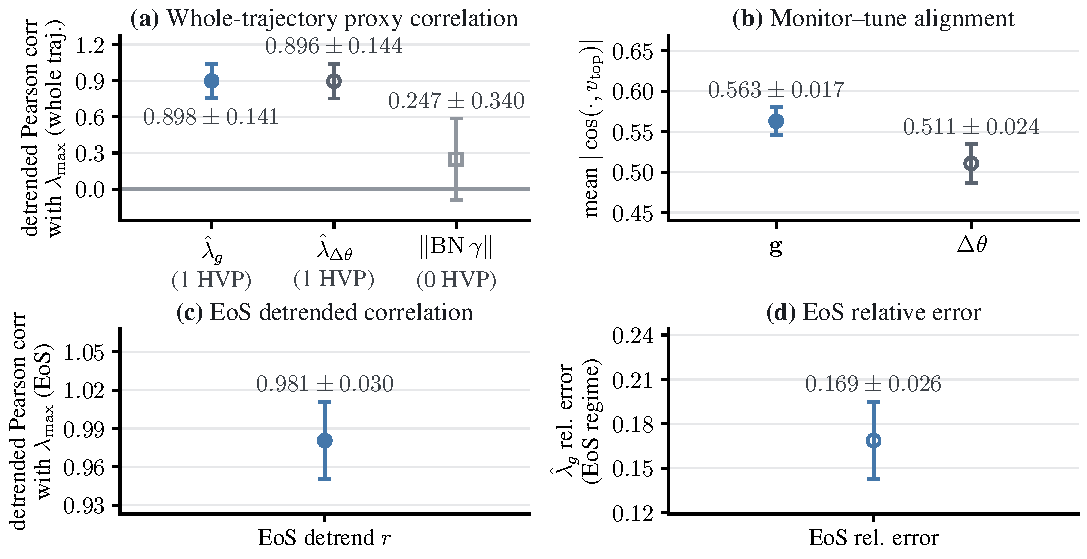
\includegraphics[width=0.9\linewidth]{fig1_rayleigh_monitor_ci.pdf}
\caption{论文图 1（$n=5$ 种子）：$\lhatg$ 是稳健的 $\lmax$ 监测器；Tier-0 的 $\gamma$ 代理种子不稳定（CI 跨零）；原始梯度 $\mathbf{g}$ 与 $\vtope$ 的对齐优于动量更新 $\Delta\theta$。}
\label{fig:ch04-rayleigh}
\end{figure}

图~\ref{fig:ch04-rayleigh} 把本章三条主张压进一张带 CI 的图里，读图时建议按
误差棒而非按均值读：$\lhatg$ 相关系数的种子间散布窄（$\pm0.030$ 量级），与
BN-$\gamma$ 横跨正负的宽 CI 形成对照；对齐面板里 $\mathbf{g}$ 与 $\Delta\theta$
两组误差棒的\emph{不重叠}，正是上面这组对比能当结论而不仅是趋势的全部统计依据。

\subsection{与教程第 9 节的衔接：从入门代理到完整地图}
\label{sec:ch04-practice}

最后把本章放回教程的延长线上。教程第 9 节的结论是“$\lmax$
太贵，权重范数可以当代理”——一个在 tanh MLP
上完全成立的入门命题。论文这一节把它升级为三件事：\textbf{(a)} 代理不止一种，按
HVP 成本排成阶梯；\textbf{(b)} 每层的可靠性是归一化族与训练阶段的函数（plain
范数、BN-$\gamma$、LN 的 $\|\mathbf{g}\|$ 各管一段，且都不稳）；\textbf{(c)}
甜蜜点是单 HVP 的 $\lhatg$，其偏差结构（瑞利 slack）被显式刻画。

由此可以写出论文隐含的\textbf{实践决策表}：
\begin{itemize}
  \item \textbf{训练中后期、已进入 EoS 对齐区}（$|\cos(\mathbf{g},\vtope)|$
高，可由 $\lhatg/\lmax$ 的稳定性侧面印证）：直接信任 $\lhatg$——$+0.981\pm0.030$
的相关加上可预测的约 $17\%$ 瑞利折减，一次 HVP 换一个近乎精确的监测器。
  \item \textbf{训练早期或归一化主导区}（对齐尚未建立）：$\lhatg$
的下界性质会使它系统性偏低且无对齐先验可校准，此时用 $\|\mathbf{g}\|$
兜底（LN/Transformer 上 $+0.52$，且对所有归一化族都是免费量）。
  \item \textbf{BN 网络}：不要在单 seed 上对 $\|\gamma\|$
下任何结论（$+0.247\pm0.340$ 跨零）；宁可付一次 HVP。
  \item \textbf{任何比较代理的实验}：密集采样，勿在 16
点量级的稀疏序列上比相关（窗口摆动可达 $\pm0.25$）。
\end{itemize}

还应注意本章在全文论证中的位置：它建立的“预测端成功”越扎实，后面控制端的失败就越有分量——\textbf{正因为
$\lhatg$ 能以 $+0.981$ 的精度\emph{读出} $\lmax$，用它去\emph{改写} $\lmax$
的失败才不能归咎于“没测准”}。预测器与执行器的分界线，是在预测器最好的位置上画出来的。

\subsection*{本章要点}
\begin{itemize}
  \item 代理阶梯三层：0 HVP 范数 / $\gamma$ 代理（归一化族依赖：plain
$\to\|\mathbf{W}\|$、BN $\to\gamma$、ViT $\to\|\mathbf{g}\|$）$\to$ 1 HVP 的
$\lhatg$ $\to$ 约 5 HVP 的热启动精确测量；甜蜜点是 $\lhatg$。
  \item Tier-0 的三个裂缝：plain 上 last-hidden 最优（$10/14$）但只到
$0.65$--$0.71$；BN 下范数相关由正转负（$-0.8$）、$\gamma$ 接棒但多种子
$+0.247\pm0.340$ 跨零；LN 上所有零计算代理挤在 $0.44$--$0.52$，且 16
点去趋势相关可因窗口摆动 $\pm0.25$。
  \item $\lhatg$ 在二次型下代数等于 $\lambda_c$（Kalra 等 2026，非本文新颖），是
$\lmax$ 的瑞利下界；ResNet 上全程 $+0.898\pm0.141$、EoS
体制（$|\cos|>0.7$）$+0.981\pm0.030$。
  \item 约 $17\%$ 的相对差距 = 瑞利下界的预期 slack（对齐 $0.85$--$0.9
\Rightarrow \cos^{2}\!\approx\!0.8$），有方向、可校准，不是噪声。
  \item 监测探针用原始梯度而非动量更新：对齐与 EoS 误差的 CI 均不重叠（$0.563$
对 $0.511$；$0.169$ 对 $0.238$），全程相关打平（约 $0.90$）——与 CDAT / Kalra
的更新方向用法形成正交分工。
\end{itemize}
